\documentclass[options]{article}

% para que traduzca las cosas por defecto del programa a español (ej: abstract -> resumen)
\usepackage[spanish]{babel}
% para insertar imágenes
\usepackage{graphicx}
% para poner headers a las tablas
\usepackage{makecell}
\renewcommand\theadfont{\bfseries\sffamily}

\title{Práctica del Tema 5: Publicación y difusión}
\author{Blanca María Pérez Soriano}

\begin{document}
\maketitle
\begin{abstract}
    \begin{center}
        Creación y publicación de un modelo 3D a partir de un modelo digitalizado representado como una nube de puntos
    \end{center}   
\end{abstract}

\pagebreak

\section{Preparación}
\subsection{Software}
%TODO: meter meshlab en un link a su página principal
Para realizar esta práctica utilizaremos el programa MeshLab en la versión 64bit v2023.12.
\subsection{Modelo de puntos}
Para la realización de esta práctica se utilizará el modelo de nube puntos proporcionado en el recurso \textit{``Modelos para la práctica"}: \textbf{MayanSculpture.ply}.
\subsection{Importación a MeshLab}
%TODO: sustituir y poner el nombre modelo que se va a utilizar
Para importar el modelo de nube de puntos seleccionado seguiremos las siguientes acciones: \textbf{File → Import Mesh → MayanSculpture.ply}
\begin{center}
    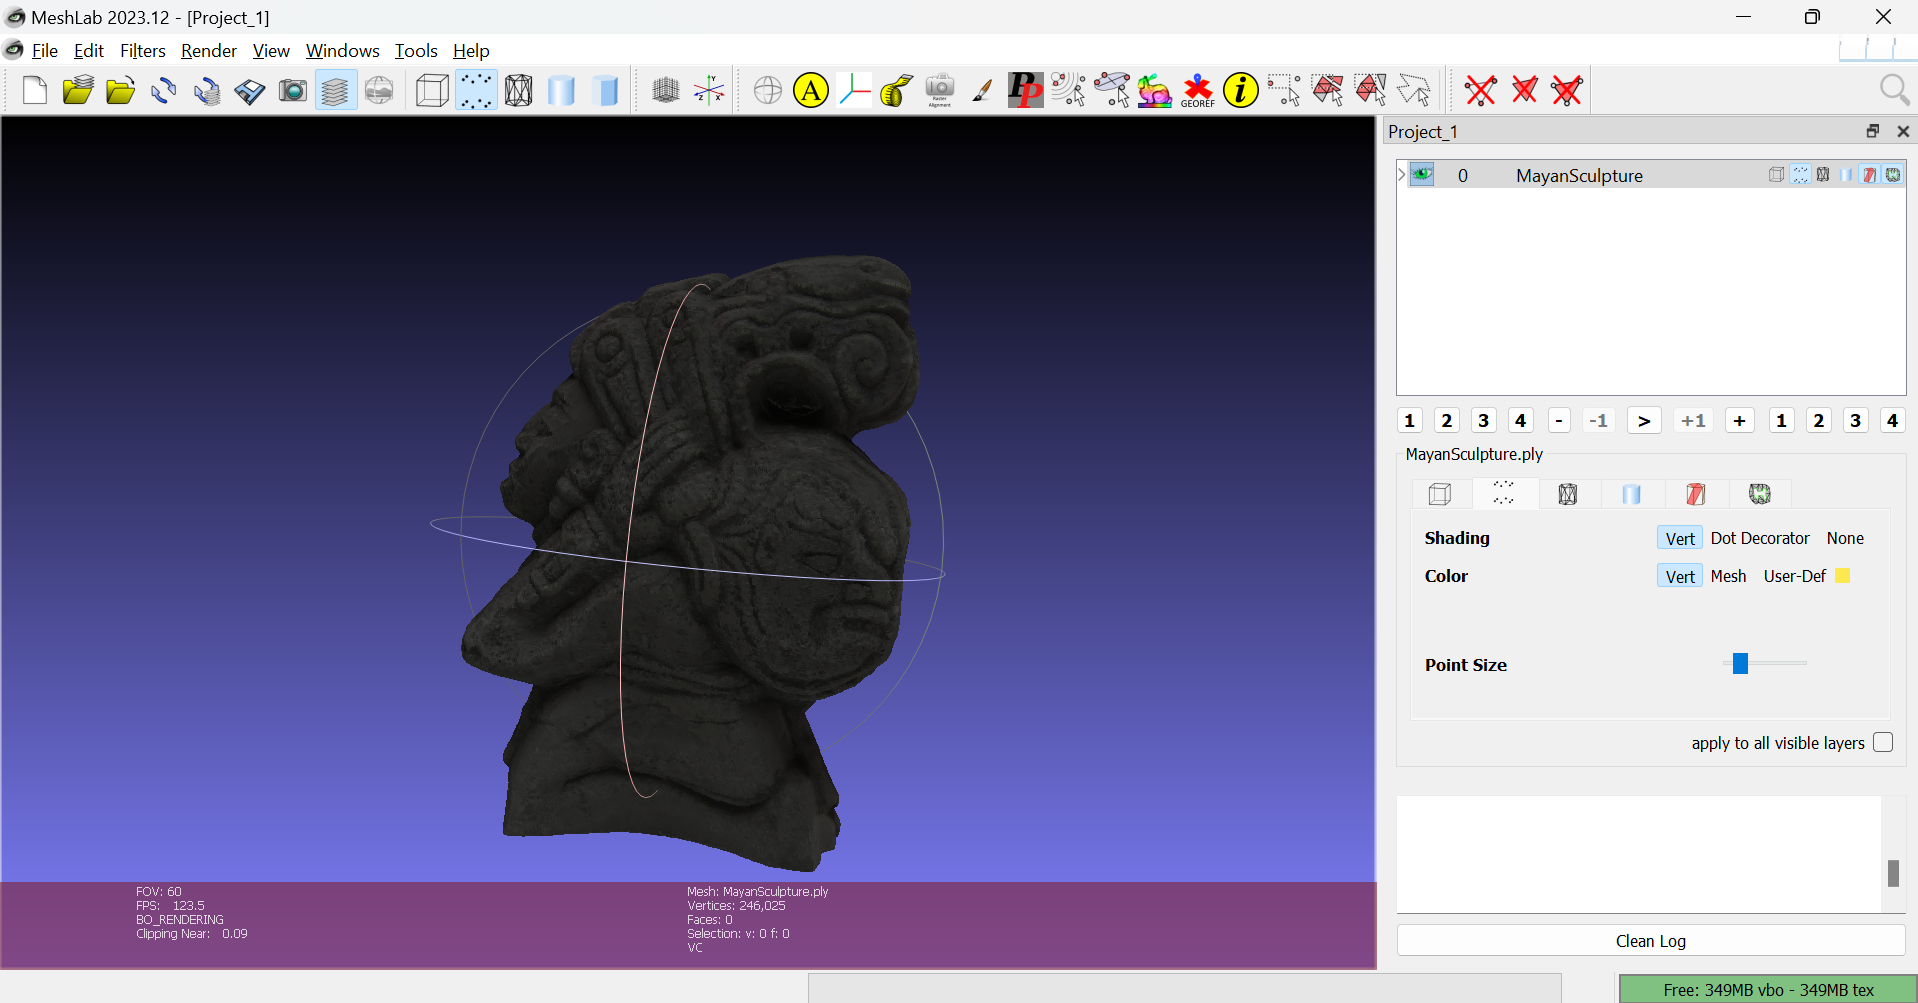
\includegraphics[scale=0.35]{images/presentacion_importacion.png}    
\end{center}

Es una maya de 246.025 vértices y no tiene caras.
\pagebreak

\section{Resolución de la práctica}
\subsection{Shading}

Para empezar correctamente, lo primero que haremos será intentar mejorar el \textit{shading} de la pieza. Para ello calcularemos las normales, esto hará que los puntos de luz sean tomados perpendicularmente. Deberemos hacer click en la siguiente secuencia: \textbf{Filters → Point Set → compute normals for point sets}. Tras esto, se nos desplegará la siguiente ventana, deberemos hacer click en \textit{``Apply''}:

\begin{center}
    \includegraphics[scale=0.65]{images/triangulación_01.png}    
\end{center}

Ahora podemos ver el claro cambio de color y trazado en la pieza:
\begin{center}
    \includegraphics[scale=0.35]{images/triangulación_02.png}    
\end{center}
\subsection{Reconstrucción de la superficie mediante Screened Poisson}

Para ello hacemos click en: \textbf{\textit{``Filters → Remeshing, Simplification and Reconstruction → Surface Reconstruction: Screened Poisson''}}. Se nos desplegará la siguiente ventana:

\begin{center}
    \includegraphics[scale=0.65]{images/triangulación_03.png}    
\end{center}

De esta ventana, los dos valores interesantes son:
\begin{itemize}
    \item \textbf{Reconstruction Depth}: este valor lo retocaremos en base a la pérdida o ganancia de puntos tras la reconstrucción.
    \item \textbf{Pre-Clean}: Este \textit{checkbox} haría un prelimpiado de normales con valores nulos, en caso de ser marcado.
\end{itemize}

Como hemos visto en el curso, un buen valor de \textbf{Reconstruction Depth} para lanzar una primera reconstrucción sería el \textbf{8}. De manera que lanzamos la reconstrucción sin tocar nada más y vemos si tenemos que reajustar. El resultado fue el siguiente:

\pagebreak

\begin{itemize}
    \item Sin pre-clean:
    
    \includegraphics[scale=0.40]{images/triangulación_04.png}    
    
    \begin{itemize}
        \item \textbf{vértices:} 135.855
        \item \textbf{caras:} 271.706
     \end{itemize}

    \item Con pre-clean: 
    
    \includegraphics[scale=0.40]{images/triangulación_05.png}
    
    \begin{itemize}
        \item \textbf{vértices:} 135.855
        \item \textbf{caras:} 271.706
    \end{itemize}
\end{itemize}

La maya original tenía 246.025 puntos, de manera que hemos reducido casi en la mitad la calidad del modelo. Podemos observar, si nos acercamos a la pieza, este tipo de pérdidas:
\begin{center}
    \begin{tabular}{|l|}
        \hline
        \thead{Por puntos} \\
        \hline
        \includegraphics[scale=0.40]{images/triangulación_06.png} \\
        \hline
        \thead{Poisson Mesh} \\
        \hline
        \includegraphics[scale=0.40]{images/triangulación_07.png} \\
        \hline
    \end{tabular}
\end{center}

\pagebreak

Repetimos el proceso aumentando el nivel de profundidad en 1. El resultado es el siguiente:
\begin{center}
    \begin{tabular}{|l|}
        \hline
        \thead{Por puntos} \\
        \hline
        \includegraphics[scale=0.40]{images/triangulación_08.png} \\
        \hline
        \thead{Poisson Mesh} \\
        \hline
        \includegraphics[scale=0.40]{images/triangulación_09.png} \\
        \hline
    \end{tabular}
\end{center}

Esta vez se han generado 546.859 vértices. A partir de aquí podríamos cambiar el color de la pieza, pero la verdad es que me gusta cómo está quedando. 

\pagebreak

Si hubiera querido cambiarlo, me habría movido entre estas dos pestañas del panel derecho, siendo la primera señalada la de los vértices y la segunda señalada la de las caras:

\begin{center}
    \includegraphics[scale=0.65]{images/triangulación_10.png}    
\end{center}

Finalmente queda eliminar algún triángulo artificial. Para ello hacemos click en \textbf{\textit{Filters → Selection → Select faces with edges larger than...}}, y el valor promedio para esta pieza es de 0.795821:

\begin{center}
    \includegraphics[scale=0.65]{images/triangulación_11.png}    
\end{center}

Tras darle a \textit{``Apply''} veo que sólo 6 caras son seleccionadas:

\begin{center}
    \includegraphics[scale=0.65]{images/triangulación_12.png}    
\end{center}

\subsection{Utilización de GitHub}

\textbf{GitHub} es una plataforma de colaboración en proyectos de software, apoyada en \textbf{Git}, lo cual nos permite llevar, además, un \textit{control de versiones} de los documentos que vayamos publicando en el repositorio. 


Para crear un repositorio y hacer seguimiento de este proyecto haremos click, dentro de nuestro panel principal, en \textbf{\textit{"New"}}:

\begin{center}
    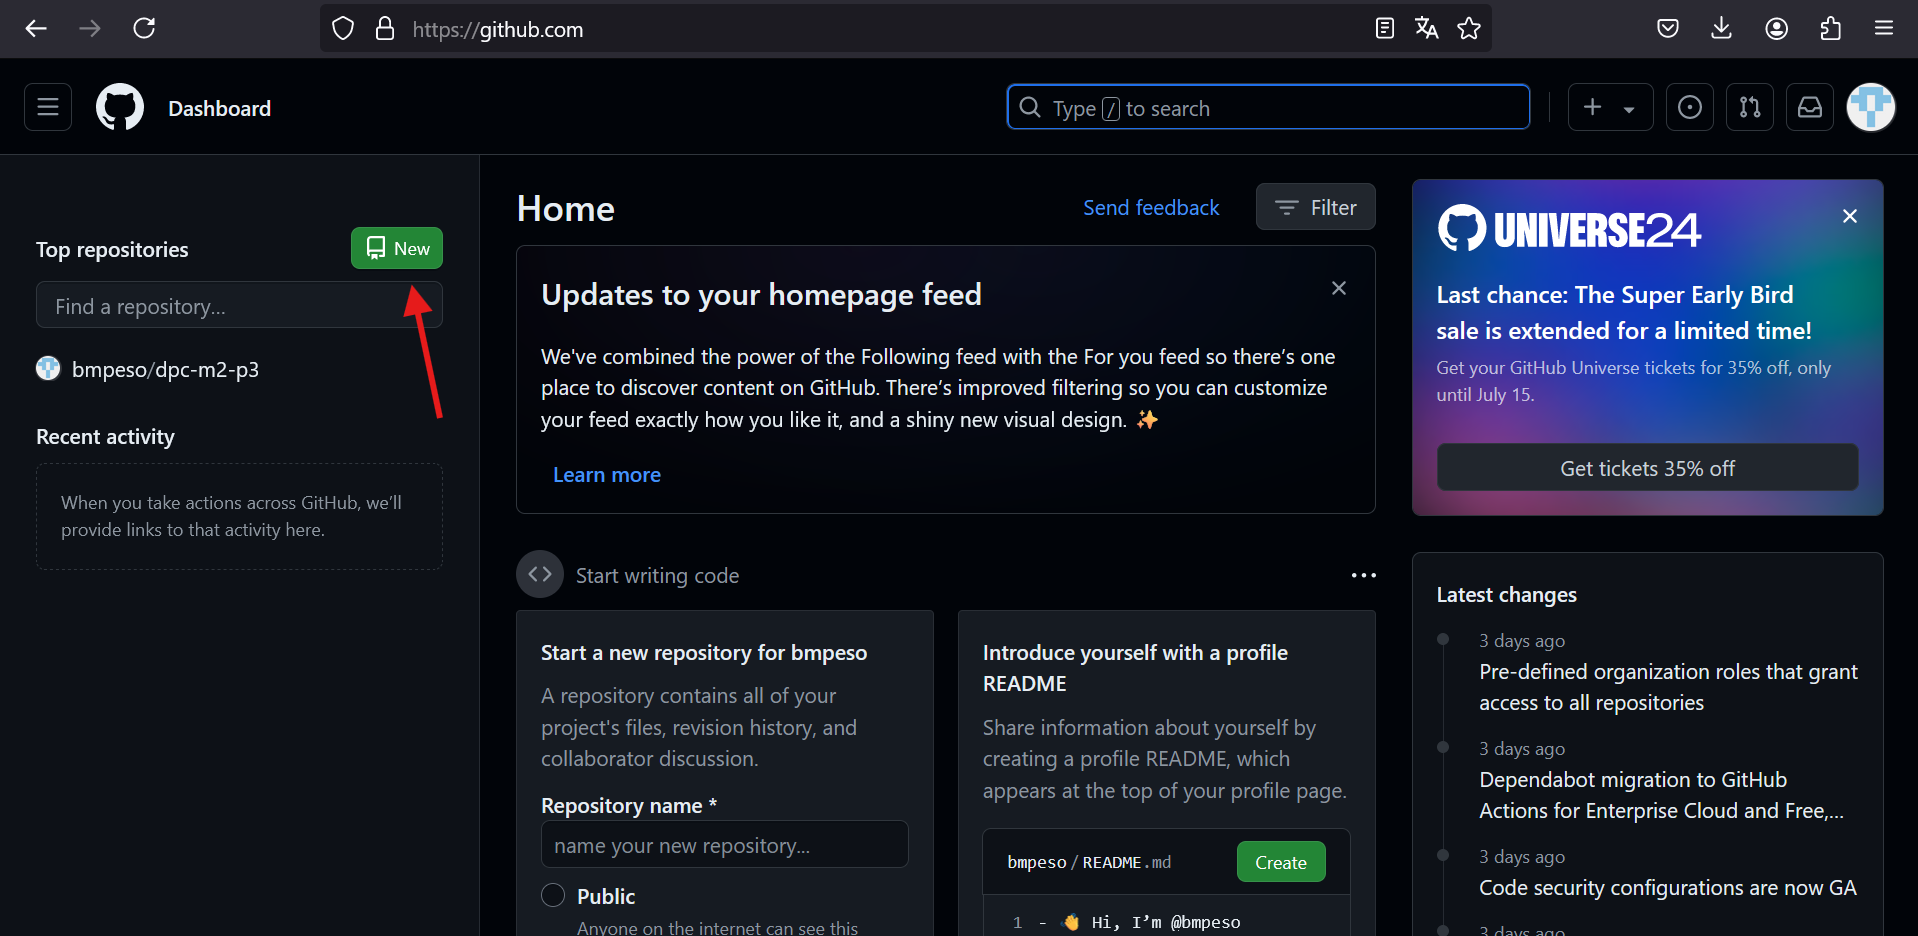
\includegraphics[scale=0.35]{images/github_01.png}
\end{center}

A continuación rellenaremos los campos que creamos convenientes \textit{(señalo en recuadros los campos modificados)} y haremos click en \textbf{\textit{Create repository}}:

\begin{center}
    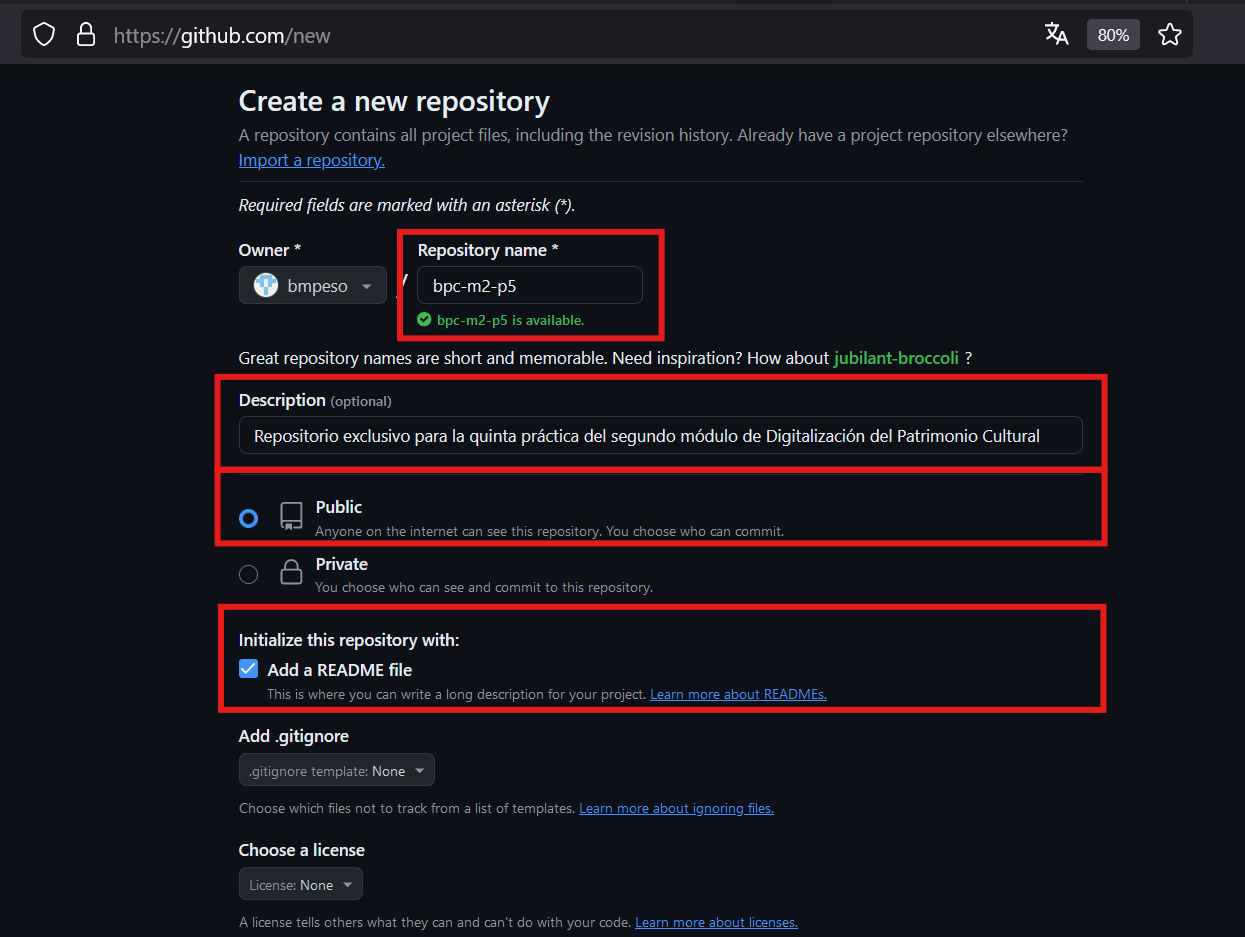
\includegraphics[scale=0.45]{images/github_02.png}
\end{center}


\end{document}